\section{Durchführung}
\label{sec:Durchfuehrung}

\begin{figure}
    \centering
    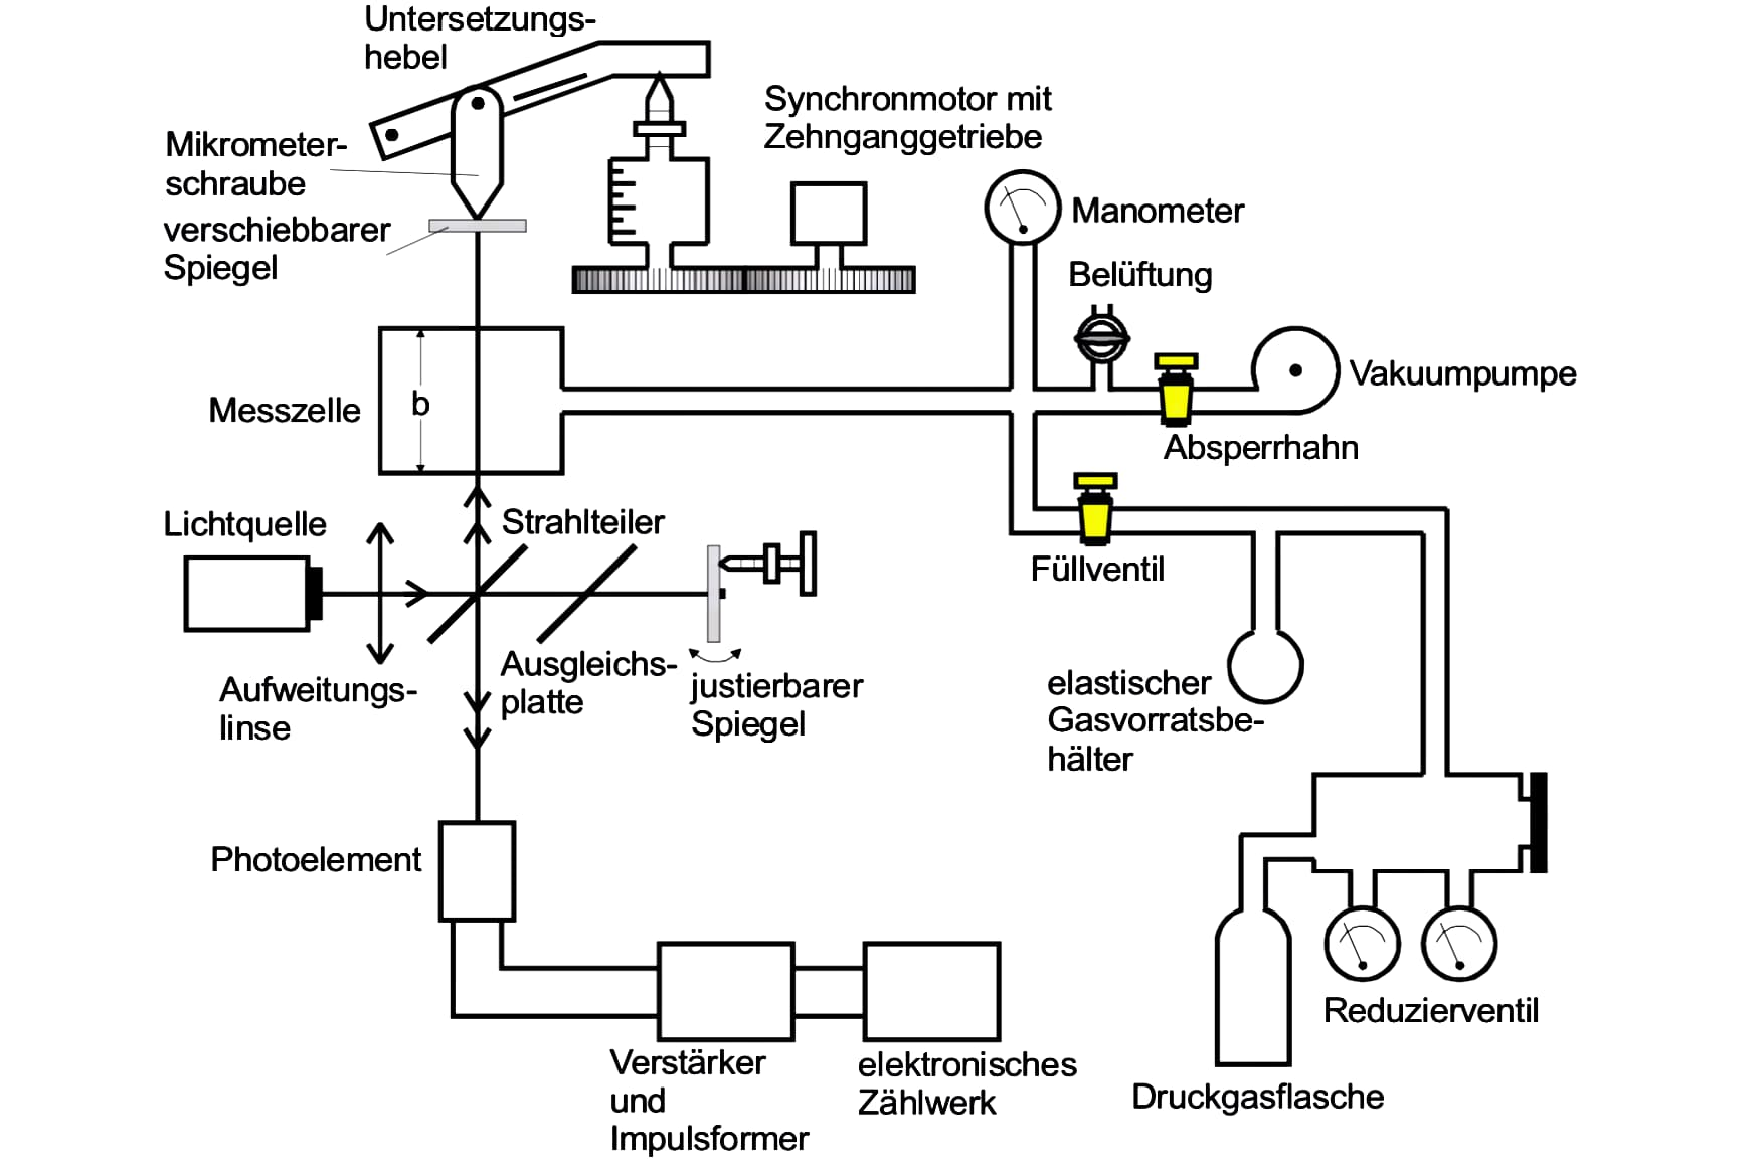
\includegraphics[scale = 0.3]{content/Aufbau1.pdf}
    \caption{Hier zu sehen ist eine Skizze zum Aufbau des Versuchs.}
    \label{fig:Teiler}
\end{figure}

Um die Wellenlänge des Lasers zu bestimmen, wird der Spiegel konstant verschoben. Dabei werden die Maxima mit dem Photoelement so lange gezählt bis die Anzahl der gezählten Maxima in etwa 3100 erreicht. Die Verschiebung des Spiegels in dem Zeitraum wird als \(d\) eingetragen.\\
Danach wird der Brechungsindex gemessen. Bei Luft wird die Messzelle evakuiert, wodurch sich der Druck sinkt. Der Druck wird daraufhin als Normaldruck eingetragen und die Messzelle mit Luft gefüllt.\\
Die Messung wird vier weitere Male durchgeführt, damit durch das Berechnen des Mittelwerts der wahre Wert angenähert wird.